\chapter{Analysis \& Design of the Solution}

The purpose of Metadata Extractor is to obtain metadata from data models created using modeling tools ER/Studio and PowerDesigner. The solution will be able to connect to Manta Flow and to bring data lineage to objects that have greater extent of abstraction than the physical ones which are currently the only objects supported by Manta.

Here we describe how we proceeded when analyzing the solution and discuss crucial features of ER/Studio and PowerDesigner in detail, so we can identify what to focus on, when implementing the tool.\\

In this chapter we seek answers for these questions:
\begin{enumerate}
	\item Identify what data models the modeling tools work with, what objects are contained in the data models, how they are organized and what metadata can be obtained that are relevant to be brought into data lineage.
	\item Find out what is the format of files that the tools save data models in. Together with how the data we assumed interesting in 1) can be reconstructed.
	\item Determine how the file format can be parsed.
\end{enumerate}

\section{Analysis of the Problem}

We already presented that the modeling tools are capable of creating data models. The output files of the tools are going to be the input of Metadata Extractor, that uses them for reconstruction of the objects and information contained in the data models.
In order to do so we needed to identify what objects the solution will look for in the files and how they are related to each other.
In \Cref{chap:database_modeling} about database modeling we introduced the standard layout of every data model type. We will quickly review the basic skeleton of each model type once again. \\

In conceptual data model is focused mainly on entities, which may have attributes. An entity may be related to other entities.

On logical layer also entities with attributes can be found and the entities may have relationships.

Physical data models are made of tables. A table belongs to a schema and is composed of columns.

These are the objects we must find in the file formats to recreate the main object hierarchy.

Then we will need to figure out how the models in maps-to relation refer to each other across levels of abstraction. For example how a logical model and a physical model, being the realization of the logical one, are tied together.

\subsection{File Format}

Firstly, we need to identify what is the output of the analyzed modeling tools, to know which what is stored in a file produced, what information are stored there, to decide what is interesting to bring to data flow and what not, and how it is done, to be able to create a software automatically reconstructing the desired information.

\subsubsection{ER/Studio}
\label{subsec:dm1_format}
The modeling tool uses its custom file format. It uses .DM1 extension. The file stores plain text and it is made up of many tables. A table in this context is a CSV (comma-separated values) structure but as there is not only one CSV table identifying name is also included. So by table we understand its name, definition of columns (or fields) and records.
How more complex objects can be stored in files like this is not clear from the first sight and it required some work to get the idea behind it. 

\begin{figure}[H]
	\centering
	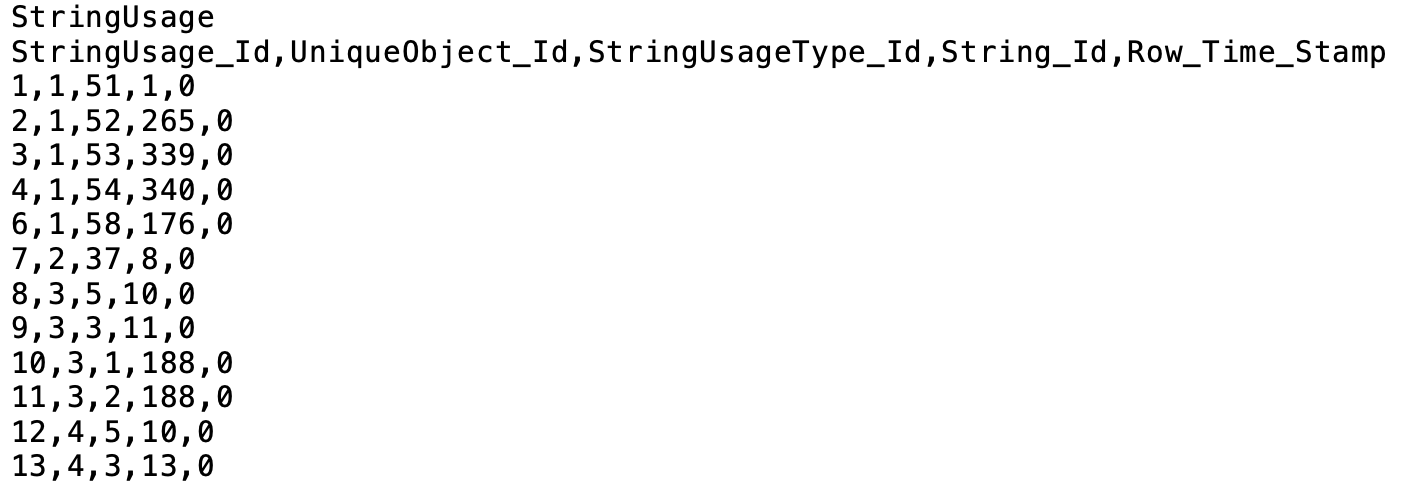
\includegraphics[width=14cm]{../img/StringUsageTable}
	\caption[CSV Table]{Example of a simple CSV table named StringUsage with five columns from a .DM1 file.}
\end{figure}


An attentive reader may find these terms, that we used for describing the data structure, familiar since we already used them where introducing relational databases. And he would be true. When investigating these tables we can notice columns that are shared, meaning relation between the tables that have them in common. This is pretty much how primary and foreign key work in relational databases.
Now we face the challenge of reverse-engineering the tables to rebuild the composite objects that are deconstructed and saved in the tables.
It would be quite exhausting to try to restore the relationships by hand, so we developed a little tool that helped us to get an overview of the format that will work on one hand with tables' metadata to find the intersecting columns as well as with the records to see whether there are similarities in data stored in different tables to uncover relations between them and the core concepts behind the file format.
Further details and ideas related to the ER/Studio file reverse-engineering tool can be found in \Cref{subsec:dm1_tool}

Surely, when we want to load an arbitrary file a component that parses it will be needed. 
We mentioned that the file of our interest is basically a sequence of CSV tables. The question was whether to reach out for an existing CSV parser or to develop a tailor made one. We took the second, option why and how we did so is described further in \Cref{subsec:dm1_parser}.

Once we understand the structure and can tell how the data we are seeking for are stored we can reconstruct them.
In one .DM1 file related data models are stored. Let's call these models a solution. An \definition{ER/Studio solution} is set of data models, describing a problem on both logical and physical levels (the two layers are only that ER/Studio supports). In a solution one logical model must be present whereas 0 to N physical ones are supporting it. 
We can imagine why ER/Studio behaves like this. The motivation may be that once there is a problem (if there is no challenge, no data modeling is needed) it is obligatory described by a logical model. Possibly user has worked out the way to solve it, and that is when physical models are present as well. 
Note that the actual storage may be distributed and the corresponding databases can be of different technologies, that is why more than one physical model is allowed in a single solution.

\subsubsection{PowerDesigner}

In the case of PowerDesigner need to handle files with three types of extensions .pdm, .ldm and .cdm. They  stand for physical data model, logical data model and conceptual data model respectively.
All of them are XML (Extensible Markup Language) based file formats.
Actually, there is an alternative to the XML files which PowerDesigner also works with. Each of the models can be saved into a binary version instead as PowerDesigner can process them more quickly. However, we need a user to save his models as XML, only this way is supported currently by Metadata Extractor.

Since we have three different output file types from the modeling tool it is easy to see that the logic of how data models are saved varies from ER/Studio's approach. 
While ER/Studio groups data models into solutions every model created in PowerDesigner is saved independently. Set of files that are currently opened in PowerDesigner form its state. Such state is called a workspace here and can be saved into a .sws file, but these files do not bring us any interesting information. The information captured stores only what files were at some time opened in the environment and does not tell anything about logical links between the captured files.

When parsing XML files there are basically two major ways we can face the problem.

The first approach is SAX (Simple API for XML) that is an event-driven parser, which process an XML document sequentially by a single pass. By default the processing is state independent and handlers are triggered when an event occurs. It is a simple (for some cases may be even too simple) and lightweight parser.

On the other hand we have a family of DOM (Document Object Model) parsers. They load an XML file into a full AST (Abstract Syntactic Tree) structure. This way of file processing is both more memory and time consuming but translates everything stored in the parsed file into data structure straightforwardly. Then we can conveniently work with the tree-like result structure where nodes represent parts of the processed document.

In the next section we describe what we want to retrieve from the PowerDesigner data model files. We will see that the objects and their properties are quite complex and composite using a DOM parser will be much more suitable and having the ability of doing XPath queries over a DOM document is nicer than having to store a context manually, what would be needed with SAX.

\subsection{Metadata to Collect from Data Models}
\label{metadata_enumeration}

The main desired feature is to to bring data lineage to the conceptual and logical level. To do this, we had to identify which metadata to collect from models on these levels.
The bare minimum is to be able to reconstruct high-level entities to have at least something to visualize data flow between, according to knowledge gained in later stages.
But we will aim to bring as much information as possible and try to make use of every relevant (meta)datum saved by a modeling tool. 
They are exhaustive pieces of software with many features and ability to capture plenty of aspects of modeled system, so we must determine what subset of the information will be extracted.
In this section we discuss what specific types of objects can we obtain and what are means to describe these objects even further by some properties of theirs. 
On the other hand we will not pay attention to relationships in entity-relationship model. This is given by nature of Manta Flow, it is not a modeling tool thus it does not work with them and links between objects are used solely to represent dependencies determined by data lineage.
The only relationship type from data models we will need to cope with is the inheritance relation. It is present in enhanced-entity-relationship models. The exception is made because if the is-a links are not captured, entities' structure are be not described completely and their attributes may be missing.
Other categories of metadata we will not extract are the ones that describe some constraints on the actual records saved in database themselves. We will work exclusively with database metadata and don't have access to what is really saved there thus we cannot neither monitor nor enforce anything on the database entries. That is why likes of keys and data types defined in data models will not be in our domain of interest.

The full list of metadata, including the ones we do not find useful to extract is listed in the appendix.

\subsubsection{Conceptual \& Logical Data Model}

Here we list objects that appear in both conceptual and logical data models, together with what additional information about them can be inserted by user.

\subsubsection{ER/Studio}

\subsubsection{CDM}

ER/Studio does not support conceptual data models.

\subsubsection{LDM}

\begin{itemize}
	\item Owner \\ 
	Owner is a concept equivalent to a schema - it is a container for logically related entities. Every entity belongs to an owner.
	\item Entity \\
	\begin{itemize}
		\item Name \\ 
		Name of an entity.
		\item Attributes \\ 
		Attributes assigned to an entity.
		\item Definition \\
		Further description of an entity. Plain text or RTF (rich text format).
		\item Note \\
		Notes are used when a documentation about an entity is generated. Plain text or RTF.
		\item Where Used \\
		Shows objects that are in maps-to relation with an entity. Those which were created by generating.
		\item User-Defined Mappings \\
		Shows objects that are in maps-to relation with an entity. These mapping are user defined. They can contain description of a relation, but we will not fetch the text as Manta Flow does not support attributes on mapping edges.
		\item Owner \\ 
		Owner an entity belongs to.
	\end{itemize}
	\item Attribute
	\begin{itemize}
		\item Name
		\item Definition
		\item Notes
		\item Where Used
		\item User-Defined Mappings
	\end{itemize}
\end{itemize}


\subsubsection{PowerDesigner}

Conceptual and logical data models in PowerDesigner have so much in common that we will propose unified view on what may be stored in them. The properties/object that are specific for either of them are marked with information in brackets saying "CDM/LDM only".

\subsubsection{CDM \& LDM}

\begin{itemize}
	\item Data Item (CDM only) \\
	A data item holds an elementary piece of information, which is given by some fact or a definition in a modeled system. It may or may not be present as a modeled object. Data items can be attached to entities to form their attributes. It is a datum that may seem relevant and is possible to capture at first but later may be not used as no entity needs it in the end.
	\begin{itemize}
		\item Name
		\item Code
		\item Comment \\
		Plain text short description.
		\item Definition \\
		An RTF description of an object.
		\item Annotation
		A further RTF description.
		\item Keywords
		Set of significant words specifying object's domain.
	\end{itemize}
	\item Entities
	\begin{itemize}
		\item Name 
		\item Attributes
		\item Code 
		\item Comment
		\item Definition
		\item Annotation
		\item Keywords
	\end{itemize}
	\item Attributes
	\begin{itemize}
		\item Name 
		\item Code 
		\item Comment
		\item Definition
		\item Annotation
		\item Keywords
		\item Parent Entity
	\end{itemize}
	\item Inheritances
	\begin{itemize}
		\item Parent Entity \\ 
		Predecessor.
		\item Child Entity \\ 
		Inheriting entity that takes over attributes of the parent.
	\end{itemize}
\end{itemize}

\subsubsection{Physical Data Model}

\subsubsection{ER/Studio}

\begin{itemize}
	\item Type of Data Model\\
	Database management system that a model is aimed for.
	\item Schema
	 \begin{itemize}
	 	\item Name
	 	\item Tables
	 \end{itemize}
	\item Table
	\begin{itemize}
		\item Name
		\item Columns
		\item Schema
		\item Definition
		\item Note
		\item Where Used
		\item User-Defined Mappings
	\end{itemize}
	\item Column
	\begin{itemize}
		\item Name
		\item Definition
		\item Notes
		\item Where Used
		\item User-Defined Mappings
	\end{itemize}
\end{itemize}

\subsubsection{PowerDesigner}

\begin{itemize}
	\item Tables
	\begin{itemize}
		\item Name 
		\item Columns
		\item Code 
		\item Comment
		\item Definition
		\item Annotation
		\item Keywords
		\item Schema
	\end{itemize}
	\item Columns
	\begin{itemize}
		\item Name 
		\item Code 
		\item Comment
		\item Definition
		\item Annotation
		\item Keywords
		\item Table
	\end{itemize}
\end{itemize}

\subsection{Recreating of Modeled Objects}

We defined what are the objects and their properties that we will try to obtain from data models. 
The objects live in the common environment of a data model, therefore they must be organized in some hierarchy.
 The above enumeration of the objects may help reader to see that the very basic layout of objects captured by a model is resembling a tree-like structure. The reason is that the basic skeleton of a data model goes like shown on the figure \TODO{figure}. A file can store one or more data models, the models may have several owners, each of them may own zero or more entities/tables which are comprised of none or multiple attributes/columns. 
 Surely further relations between the objects will come to play, like inheritances or mappings discussed later in the \Cref{maps_to_analysis}, making the diagram of actors in the system more complex.
 
 These objects can be seen then as nodes of the tree, whereas their properties are attributes of the corresponding nodes.
 
Metadata Extractor will build the tree from top to bottom. Firstly, it reconstructs the root standing for a file, then link it to its children, data models, and so on and so forth.

\subsubsection{ER/Studio}

In the case of ER/Studio, each type of the objects is defined in some table that defines its type as such table is used for storing all instance of the type. It has an id relative to its table used for identification among other realizations of the same type. Basically all links to other objects are done using foreign keys, the only necessity is to know from which tables the keys come from. 
So if an object has a reference to its, if we stick with the tree terminology, parent we can get it by looking at what is the id being referenced and identifying the reconstructed object using this information and as we are descending down the tree the object is already loaded and we can plug the child in.

\subsubsection{PowerDesigner}

XML files form a tree structure by definition what makes storing hierarchy of objects with the same nature very much natural and straightforward. 
This way a parent object of a child is simply its predecessor in layout of XML elements. 
Other properties of an object are stored as child elements as well or attributes of the object's representation. 
Also in this case creating our resulting tree structure top-down makes sense. As first, on our way from the XML root, build objects higher in the hierarchy and only if a parent is build we examine its children.


\subsection{Maps-to Relation}
\label{maps_to_analysis}

Once we identified objects across the data models, it is really useful to know which ones are related even though they are not defined at the same level of abstraction. It is important to keep the data models readable and to know what tables are implementing which high level concept.

Our tool deals only with mappings of objects which are not at the same level of abstraction. 
Some modeling tools allow mapping, for example, a logical entity to a logical but it is unclear what is the meaning of such construct, since we have relationships available for defining relationships like that. Possibly it could indicate that the objects are used identically as they are implemented by a single database table, but that is what data lineage describes precisely and will be brought by Metadata Extractor.

To be specific only the following mappings we will extract: 
\begin{itemize}
	\item An entity to a table or another entity. 
	\item An attribute to a column or another attribute.
\end{itemize}

\subsubsection{ER/Studio}

We already listed two types of mapping relation that entities, tables, attributes and columns in ER/Studio can dispose of. 
In fact their meaning is the same, the only difference is that the where used mappings are generated automatically and the user-defined are drawn by user. We assumed that all the objects in maps-to relation are in the very same solution but there is also an option to create a mapping to objects that are defined in different .DM1 files. It can be done using the Compare and Merge utility in ER/Studio whose functionality is to synchronize a model with another model/live database/SQL file. Among other operations that keep the pairs in sync there is the mapping creation option. We are interested in the first scenario where models may come from two solutions. The compared models' objects are listed side by side and mappings can be created between pairs of them. These mappings are referred to as universal. \\

Our focus is on how mappings are saved in an ER/Studio solution. \\ 

We will look at what is required to do in order to extract the mappings.
Let's start with the seemingly easier case of mappings between objects inside the same solution. After some analysis we found a CSV table defining them named Where\textunderscore Used\textunderscore PD.
In the table there are four crucial attributes, IDs of the mapped objects and their Meta table types.
The first two attributes are foreign keys to tables where the mapped objects are defined. The second pair of columns defines a type of the object so that we know to which tables we should look for the keys that are referenced. The meta tables also allows us to check if the objects are actually compatible with each other. \\

At the first sight solving the universal mappings may appear more difficult as it looks like we will need to search for object in different solution than the one that is analyzed and reconstruct them. But the way it is really solved in ER/Studio is much simpler. We don't need to go anywhere else as the external objects referenced by a mapping are saved in the solution as well. They are described briefly in a table called External\textunderscore Mapped\textunderscore Objects by XML structures.
Also a table Universal\textunderscore Mappings using the same concepts as Where\textunderscore Used\textunderscore PD allows Metadata Extractor to reconstruct them easily.

\subsubsection{PowerDesigner}

By the nature of how PowerDesigner saves every data model into a separate file to resolve mappings will be not as straightforward as in the case of ER/Studio.
So every mapping we take into account is an external one, using the terminology introduced above. There is a further division into two categories. Similarly as in the first tool, the mappings may be either generated or user-defined. \\ 

Before we will go through how they are represented we must mention the way objects taking part in the relation are identified.
Every standalone object in PowerDesigner has a unique identifier stored in its attribute named ObjectID. This sequence of characters (string) is used when referring to an object in the XML.\\

When an object is created out of an existing one it is reflected in the structure of the object's definition. In such case an element History is present where all the ids of objects that made an impact on the objects creation are listed there.

User defined mappings are stored separately. 
An XML element describes one mapping relation. The structure is formed by a pair of mapped entities/tables and if their underlying attributes/column that are in maps-to relation as well.

So we are reading a file where the mappings are defined but we are only able to reconstruct a single object in the relation out of two. 
The only property of the second one known is its id. We will need to find the object corresponding to the id in the file where it is defined in order to gather all the required metadata about it.
Thus in situation like this a data model file are somehow dependent on other(s).
To learn about the needed files, there is an XML element describing targets of a model.
When a model is generated from a file a dependency is created in both of the data model files, the one that was generated just like in the one that it was generated from. In other words, if we imagine an oriented graph where a file is a node and an edge leads from file $a$ to file $b$ $\iff$ $b$ is listed as a target file of $a$, then bidirectional edges are created when models are created by generation.
Whereas when user-defined mapping is created from an object in a source model $a$ to an object in a target model $b$, only the $a \rightarrow b$ edge is created and the $b$ file has no knowledge about the mapping.
We must solve how a resolution of the foreign objects will be done. As we have nothing but a target object's id, not even information what file does it from a naïve approach would be hugely inefficient. 
It would go search for every demanded id across all targets. 
But that potentially leads to a great amount of file opens as well as having to reconstruct the same objects over and over, leading to a big time overhead.
Surely we can improve this solution by collecting the ids and postponing the resolution to the and so when processing a single files its target would be opened only once and the reconstruction of the object would take place one time as well. But that is still expansive in terms of time.
If we went in a different direction and processed each of the model once, then stored all the objects that may be referred to and once all the data models on input are loaded, resolve mappings. Logic like this would decreased count of reconstructions and file openings to ideal amount but eventually, if number of inputted data models would be too big the size of memory claimed by Metadata Extractor could become unbearable.
To achieve a solution that would have advantages of the both naïve approaches we need to split the set of input files into disjoint subsets that represent the smallest group of logically tied files. We will transform all of the unidirectional edges in the dependency graph described above into bidirectional and will find connected components, that will be our searched logical groups. Therefore we can make the resolution at the end as storage requirements for objects of such subset should be reasonable enough. Based on the assumption that the far most common use-case is having three data models - logical, conceptual and physical (or few physical ones). \\

\begin{figure}[H]
	\centering
	\begin{center}
		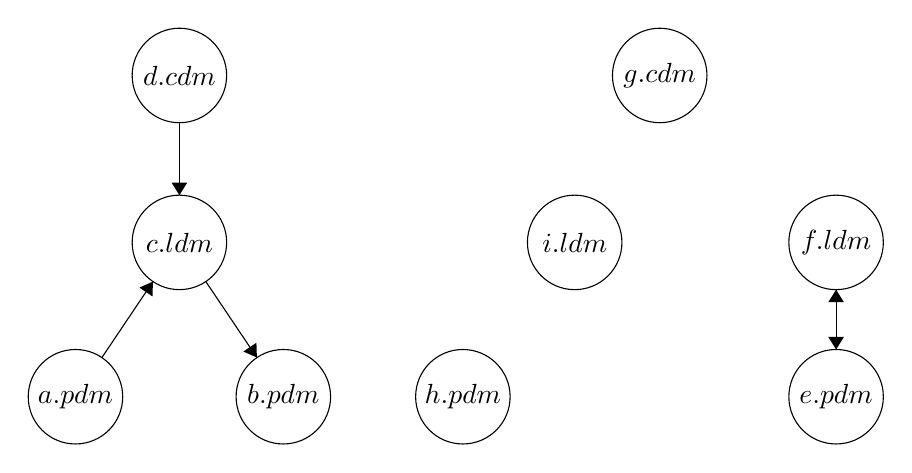
\begin{tikzpicture}[scale=0.2]
		\tikzstyle{every node}+=[inner sep=0pt]
		\draw [black] (7.9,-32.9) circle (3);
		\draw (7.9,-32.9) node {$a.pdm$};
		\draw [black] (21.1,-32.9) circle (3);
		\draw (21.1,-32.9) node {$b.pdm$};
		\draw [black] (14.5,-23.1) circle (3);
		\draw (14.5,-23.1) node {$c.ldm$};
		\draw [black] (14.5,-12.5) circle (3);
		\draw (14.5,-12.5) node {$d.cdm$};
		\draw [black] (56.2,-32.9) circle (3);
		\draw (56.2,-32.9) node {$e.pdm$};
		\draw [black] (56.2,-23.1) circle (3);
		\draw (56.2,-23.1) node {$f.ldm$};
		\draw [black] (45,-12.5) circle (3);
		\draw (45,-12.5) node {$g.cdm$};
		\draw [black] (32.5,-32.9) circle (3);
		\draw (32.5,-32.9) node {$h.pdm$};
		\draw [black] (39.6,-23.1) circle (3);
		\draw (39.6,-23.1) node {$i.ldm$};
		\draw [black] (9.58,-30.41) -- (12.82,-25.59);
		\fill [black] (12.82,-25.59) -- (11.96,-25.97) -- (12.79,-26.53);
		\draw [black] (16.18,-25.59) -- (19.42,-30.41);
		\fill [black] (19.42,-30.41) -- (19.39,-29.47) -- (18.56,-30.03);
		\draw [black] (14.5,-15.5) -- (14.5,-20.1);
		\fill [black] (14.5,-20.1) -- (15,-19.3) -- (14,-19.3);
		\draw [black] (56.2,-26.1) -- (56.2,-29.9);
		\fill [black] (56.2,-29.9) -- (56.7,-29.1) -- (55.7,-29.1);
		\draw [black] (56.2,-29.9) -- (56.2,-26.1);
		\fill [black] (56.2,-26.1) -- (55.7,-26.9) -- (56.7,-26.9);
		\end{tikzpicture}
	\end{center}
	\caption[PowerDesigner Components Example]{On the example we have four five  components made of PowerDesigner data models. If dependencies of data models are like this, a.pdm should get processed and resolved in one batch with b.pdm, c.ldm and d.cdm. Then f.ldm must be handled with e.pdm, while rest of the models are independent and form component of size one. }
\end{figure}

But there is one more matter remaining that may cause some problems. The basic scenario how a user will behave is that he will works with PowerDesigner data models in some directory, for example C:/PowerDesigner/Project/ and once he wants to let them analyze by Metadata Extractor he drags them to a different directory, that is used as input for our tool.
This way, the paths pointing to targets of models became are not correct since they have no reason to be updated and still depend on the files in C:/PowerDesigner/Project/. We want to work only with the files that user explicitly marked as to process, those are only the ones that are present in the input directory. Also if this problem is not thought of, it may cause undesired and unexpected behavior. 
For example we have file $a$ referring to $b$ in input but a change of external object in C:/PowerDesigner/Project/$b$ would have affect on $a$.
So we will try to come up with a fallback for this situation and will try to deduce by the former path the one in input folder.
As first, we will try the ideal scenario and check whether the target is in the input directory. If yes, we are done with this one.
If not we will assume similar structure of the both directories and that the names of files were not changed.

\subsection{Business Lineage Creation}
The ultimate goal of the work is to develop a tool capable of creating business\footnote{By business lineage we mean data lineage that is formed on a higher level on abstraction than on the physical level.} data lineage automatically.
We decided to build the high level lineage based on the physical one since it provides the most precise foundation in terms of correctness as it captures the real data movement in a live database.
Manta Flow primarily analyzes physical data flow but there is already implemented a functionality which can propagate the lineage to objects that are mapped to the physical objects taking part in it.
In our domain by \definition{interpolation} we mean the process of making data flow edges based on information given by lower layer.
We must ensure the objects we collect in physical data models are correctly merged as described in \Cref{matching_physical_objects} to make the most of the interpolation.

\begin{figure}[H]
	\centering
	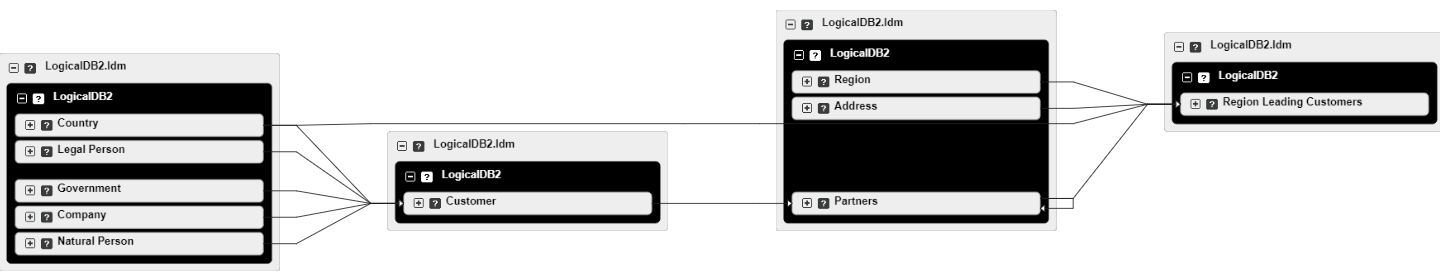
\includegraphics[width=14cm]{../img/BusinessLineage}
\end{figure}

\begin{figure}[H]
	\centering
	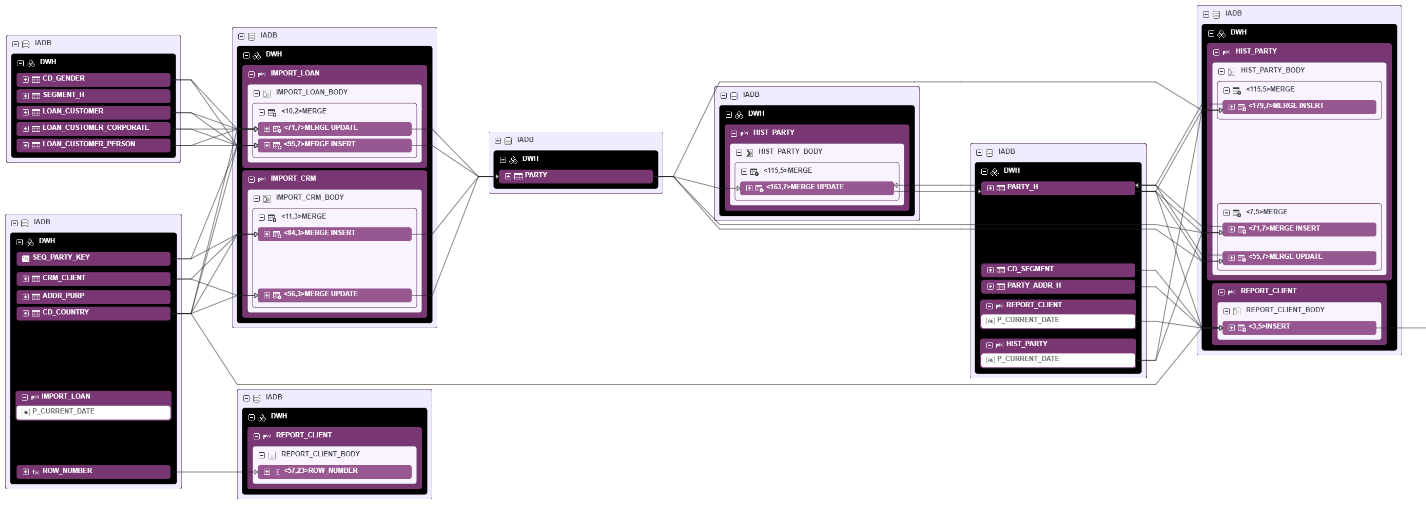
\includegraphics[width=14cm]{../img/TechnicalLineage}
\end{figure}

The two visualization of data lineage show the very same database system from two different perspectives. The business lineage hides transformations and speaks natural language, using concepts that appear in real world providing cleat motivation of the business process. 
Whereas technical data lineage precisely illustrates what happens with data in a database management system.
\TODO{where to put this, describe the mappings visually or verbally?}
\subsection{Database Connections}

Modeling tools usually can make connections to a databases. It is useful for multiple reasons. For example already familiar reverse-engineering would not be possible without this ability since metadata are fetched directly from a database in order to capture its most up-to-date state. Also one of the features of modeling tools is keeping data models and databases that are tied with them in sync, so basically there is a mechanism for comparing actual state of a database with a model. 

Manta Flow also extracts metadata of databases for needs of data lineage creation. It is done via JDBC connections.

What we will do is not accessing metastores \footnote{Shortly for metadata storage} of databases. Getting metadata directly is not really straightforward as each database technology has its own specifics - type of metadata and their organization varies greatly. Instead we will make use of the fact that Manta does has connectors that do the job for us, stores the metadata in its own local database and has unified API for getting the metadata independently of database engine. 

And why would we want to request another metadata when that is just what we are extracting from physical data models? \label{matching_physical_objects}
Because we are interested in data lineage which it is created by Manta Flow based on the real metadata of physical objects that are present in database.
The simple view is that at the moment when we ask for the objects from Manta Flow's metastore, the analysis of data flow has already taken part, thus there are data lineage edges leading between the objects. To bring together both features of Manta Flow and our tool, that brings more metadata and links to higher abstraction data models, we need to merge equivalent physical objects which come from the both sources - from Manta's extraction as well as from our tool. 
So only if we are on the same page and we know what database at which server the modeled objects belong to we can ensure correct pairing of the objects and data lineage. \\

The details we use for identification of a database instance are the following:
\begin{itemize}
	\item Database Type (Technology)
	\item Database Name
	\item Server Name
	\item Schema Name
	\item User Name
\end{itemize} 
All the above can be stored in one property called \definition{connection string}.\\
To this set of properties we will refer as a \definition{connection}. \\
As each physical data model describes a single database (or its subset) we need exactly one connection for each processed physical model in order to achieve what we described just above.

\subsubsection{ER/Studio}

Databases whose models are created in ER/Studio can be reached only by ODBC drivers present in the used machine.

We cannot really work with that, so we will leave it up to a user to define connection parameters by hand.
A .ini files \label{ini_connections}is used for that where sections are named by physical models that they correspond to and connection details are specified inside a section. 

The tool tries to get as much information as possible from an ER/Studio data model, however name of a database and server must be added manually by a user as the tool does not save these data.

\subsubsection{PowerDesigner}

In PowerDesigner a user has multiple options for connecting to a database to choose from. Either ODBC or JDBC connection may be used. 
We would like to have the ability to find out what connections with what parameters were used for connecting to a database corresponding to a physical model. So a great help would be if there was a trace left after every each connection is made. We cannot enforce it but in PowerDesigner these traces can be created when connecting using .dsn or .dcp files.
The tool has nice user environment for creating or using connections to a database where a user is guided through set up nicely and can test if he did set up everything correctly. \\

The .dsn files are definitions of ODBC connection containing parameters for an ODBC driver and stores all the interesting information we would like to have. The drawback of this file format is that it varies from a technology to technology. It has a structure of an .ini files but the properties representing the same concepts may be called differently. That means we would need to have a parser for each supported database engine. \\

On the other we have .dcp files. They can store information about native DBMS connection or about JDBC connection. 
The nice fact about them is that they are not that flexible and once we know whether we deal with native or JDBC respectively we know what exact structure expect. 
It is also a file consisting of property=value map.
There are couple of properties common for both types, like description and user name.
Then the most important property of a JDBC .dcp file is JDBC connection URL - in other words connection string which should sufficiently define a connection.
In case of native DBMS variant Server Name along with Database Name are crucial in order to identify a database we are connecting to by the setup.

But there is a problem that is common for both of the approaches, namely that there is no link between the connection file and a model that is result of reverse-engineering of the connection. So we will stick with the same solution using auxiliary .ini files as in the case of ER/Studio which is also standard for Manta Flow \Cref{ini_connections}.

\subsection{Output Representation}

The output of Metadata Extractor will be a graph. Earlier we discussed what are going its nodes and edges stand for. The remaining part is how we will represent the output. We require a structure that is both convenient to work with programmatically as a data structure and able to be visually presented to a user of our tool.
Also we must take into account that Metadata Extractor is going to be plugged into an already existing software environment. 
Manta Flow is backed by a database storing graphs of data lineage. There is already an existing browser-based user interface using which the data flows can be shown and previewed interactively. Given that we would like to comply with the graph database and merge our graphs to the storage and having the ability to reuse the visualization for presentation of the outputs, the most natural solution is to stick with the very same representation of graph as Manta does.
In the alternative scenario when we don't want to let Manta handle the output, there is a possibility of using a writer which produces an image of the output at local machine, in contrary of sending it to the Manta Server where the graph database is.


\section{Requirements/Desired Features}

To summarize the analysis, the overall goal of the developed software is to collect metadata that will allow it recreate physical, logical and conceptual modeled objects with all attributes that may be interesting when shown in data lineage. \\ 

The analysis forms a set of functional requirements or features we want Metadata Extractor to have.

\begin{itemize}
	\item Load objects from data models and reconstruct their hierarchy.
	\begin{itemize}
		\item ER/Studio: Logical data model \& physical data model.
		\item PowerDesigner:  Conceptual data model, logical data model \& physical data model.
	\end{itemize}
	\item Resolve mappings leading between objects originating in different data models.
	\item Match the loaded physical objects with their equivalents extracted by Manta Flow if possible, in order to bring in the physical data lineage they take part in.
	\item Create a graph out of the loaded structure. \\
	So that it can be further:
	\begin{itemize}
		\item Displayed in the user interface of Manta.
		\item Printed to a file as image.
	\end{itemize}
\end{itemize}


\section{Survey of Existing Solutions}

We are working on development of an automated solution that delivers business lineage.
In order to justify that we are not reinventing a wheel let's have a look at the software can provide similar functionality as Metadata Extractor.

The competitors can be divided into multiple categories:

\begin{itemize}
	\item Data Governance Frameworks \\ 
	\definition{Data governance} is a discipline that helps enterprises to gain control over their data. Commonly data lineage is a part of functionality that data governance solutions provide. \\
	Usually the solutions work with \definition{business glossary} which is a set of terms used in business together with their definitions specifying what they precisely mean in a domain. It unifies a vocabulary between system's stakeholders to avoid misinterpretations when it comes to high-level terms. 
	\begin{itemize}
		\item Collibra \\ 
		Works with business assets that connects business terms from glossary to data assets (eg. database column or table). The connections are established manually\cite{CollibraBusinessAssets}. In data lineage diagram business terms can be displayed along with the related data assets to ensure better traceability\cite{CollibraVisualization}.
		\item Informatica Axon \& EDC \\ 
		The solution by Informatica Corporation works on a very similar base as the previous one.
		Data assets are connected by hand in a user interface to business glossary entries\cite{InformaticaBusinessAssets}. That allows, once a technical data lineage is created, to drill down to the data lineage going thorough the mapped database elements. In the data flow can be also found related business assets next to related tables.
		\item IBM IGC \\ 
		IBM approaches to data lineage in such way that it only displays assets that should be relevant for a business user. In fact it is just a subset of technical lineage and what is shown is picked by a user \cite{IbmIgcBusinessLineage}.
	\end{itemize}
	\item Data Lineage Tools \\ 
		A data lineage company asg technologies company seem to do something with modeling tools as they apparently dispose of connectors for some modeling software. However no appropriate documentation can be found and the latest update traceable on ER/Studio connector was made in early 2014. \cite{AsgErStudio}
		The supported version of ER/Studio is 9.7, while the version 18.0 is out today.
		Similarly with their PowerDesigner connector, it is not easy to find a documentation and even if something related is mentioned the information seem to be obsolete nowadays.
	
	\item Modeling tools \\
	Both of the analyzed tools, ER/Studio and PowerDesigner, have means to create something like data lineage models, or lineage can be specified by mappings in a single data model. The problem with this approach is that it is not based on an analysis of SQL code managing the database and the approach is not automated. Creating such models is exhaustive and error prone as a user has to define the flow all by himself. 
\end{itemize}


To our knowledge none of the solutions disposes of the automated functionality we aim to provide by putting together Modeling Tools, Manta Flow and finally Metadata Extractor. That is to create an abstraction over technical details of databases, summarizing the real data flow using business vocabulary.

\section{Architecture of the System}

Metadata Extractor consists of two major parts where the first one handles ER/Studio models and the second one processes PowerDesigner files.
Further division of each of the parts is that they are split into four modules forming a system. 
Then the most high-level view of the system's architecture is following:
\begin{itemize}
	\item Model \footnote{There is a naming collision but here we don't refer to any data model but a data structure that reproduces objects stored somewhere, which one of these two possible meanings we use should be clear from context.}\\ 
	Is a read-only description of a data model source. On one hand it reflects the raw structure of a file so no information is left out when compared to the source. 
	On the other hand it allows reading access to the modeled objects we are interested in that were reconstructed in convenient fashion.
	\item Resolver \\ 
	Is the part where the logic of construction of objects from a file is hidden and loading of the model is done. 
	\item Reader \\
	Puts together the model and resolver unit - creates a model from a parsed structure of a file using the resolver and hands the result to the data flow generator.
	\item Data Flow Generator \\ 
	Creates a graph representation of a model \ref{model_data_structure}. Communicates with Manta Flow via its API to pair modeled objects with database objects extracted from live databases, based on a correct pairing interpolation is done.
	\item Manta Flow \\
	The external part capable of crating data lineage on database objects.
\end{itemize}
\TODO{A figure showing cooperation of the most important components }